\subsubsection{Descripción y grafo de relación entre los nodos}

Nuestro primer experimento consistió en medir la LAN Wi-Fi pública del shopping Alto Palermo. Esta medición se llevó a cabo un día Sábado a las 21hs, el tiempo de medición fue de aproximádamente 40 minutos y se capturaron 1569 paquetes ARP, de los cuales 687 eran de tipo \emph{who-has}.

Sin embargo, para graficar decidimos usar sólo los primeros 400 paquetes capturados, ya con una cantidad tan grande de paquetes, los gráficos eran poco legibles.

A continuación mostramos un grafo que muestra los nodos de la red con su dirección IP y la cantidad de mensajes de tipo \emph{who-has}.

\begin{figure}[H]
 \begin{center}
  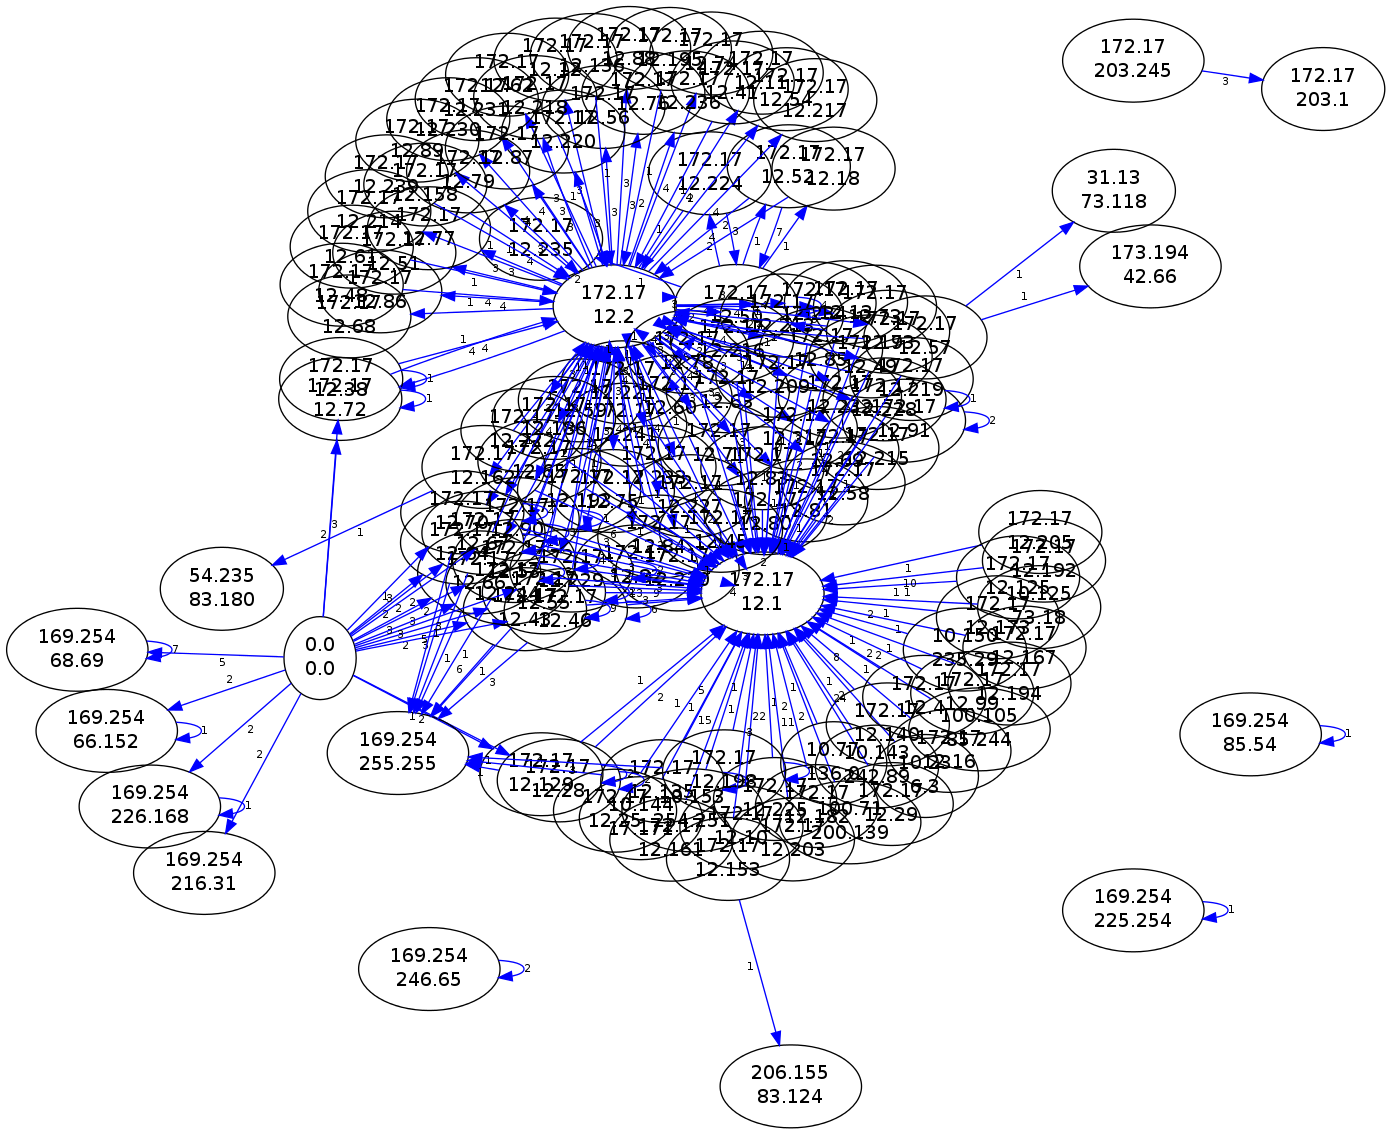
\includegraphics[width=0.9\linewidth]{../imgs/red-alto-palermo_red.png}
  \caption{Grafo Medición Alto Palermo}
 \end{center}
\end{figure}

Como podemos ver en el grafo, la red tiene dos nodos que se destacan. Uno de estos nodos, el cual tiene la dirección IP \emph{117.17.12.1}, recibe muchos paquetes de la mayoría de los otros nodos de la red, pero no envía ninguno. Y el otro recibe varios paquetes y también envía varios.

También podemos observar que hay un nodo con dirección \emph{0.0.0.0}, el cual envía varios mensajes. %TODO explicar qué es el 0.0.0.0

\subsubsection{Fuente: $S_{dst}$}

A continuación incluimos el histograma y el gráfico de información de la fuente $S_{dst}$. 

\begin{figure}[H]\centering
  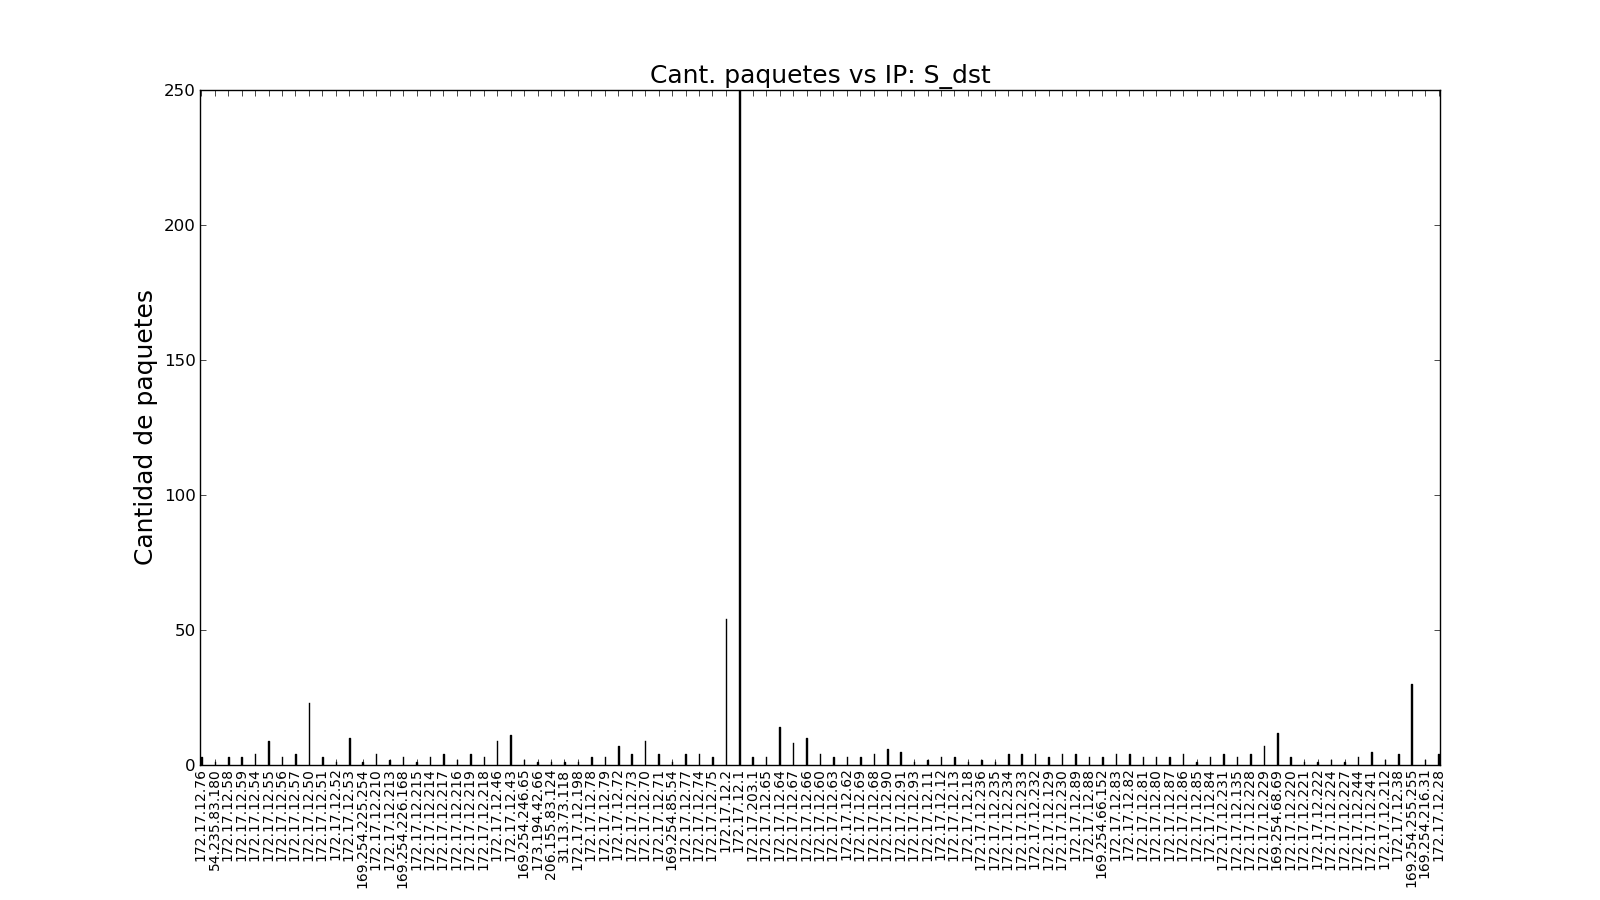
\includegraphics[width=0.8\linewidth]{../imgs/red-alto-palermo_S_dst_hist.png}
  \caption{Histograma de $S_{dst}$}\label{fig:Alto-dst-hist}
\end{figure}

\begin{figure}[H]\centering
  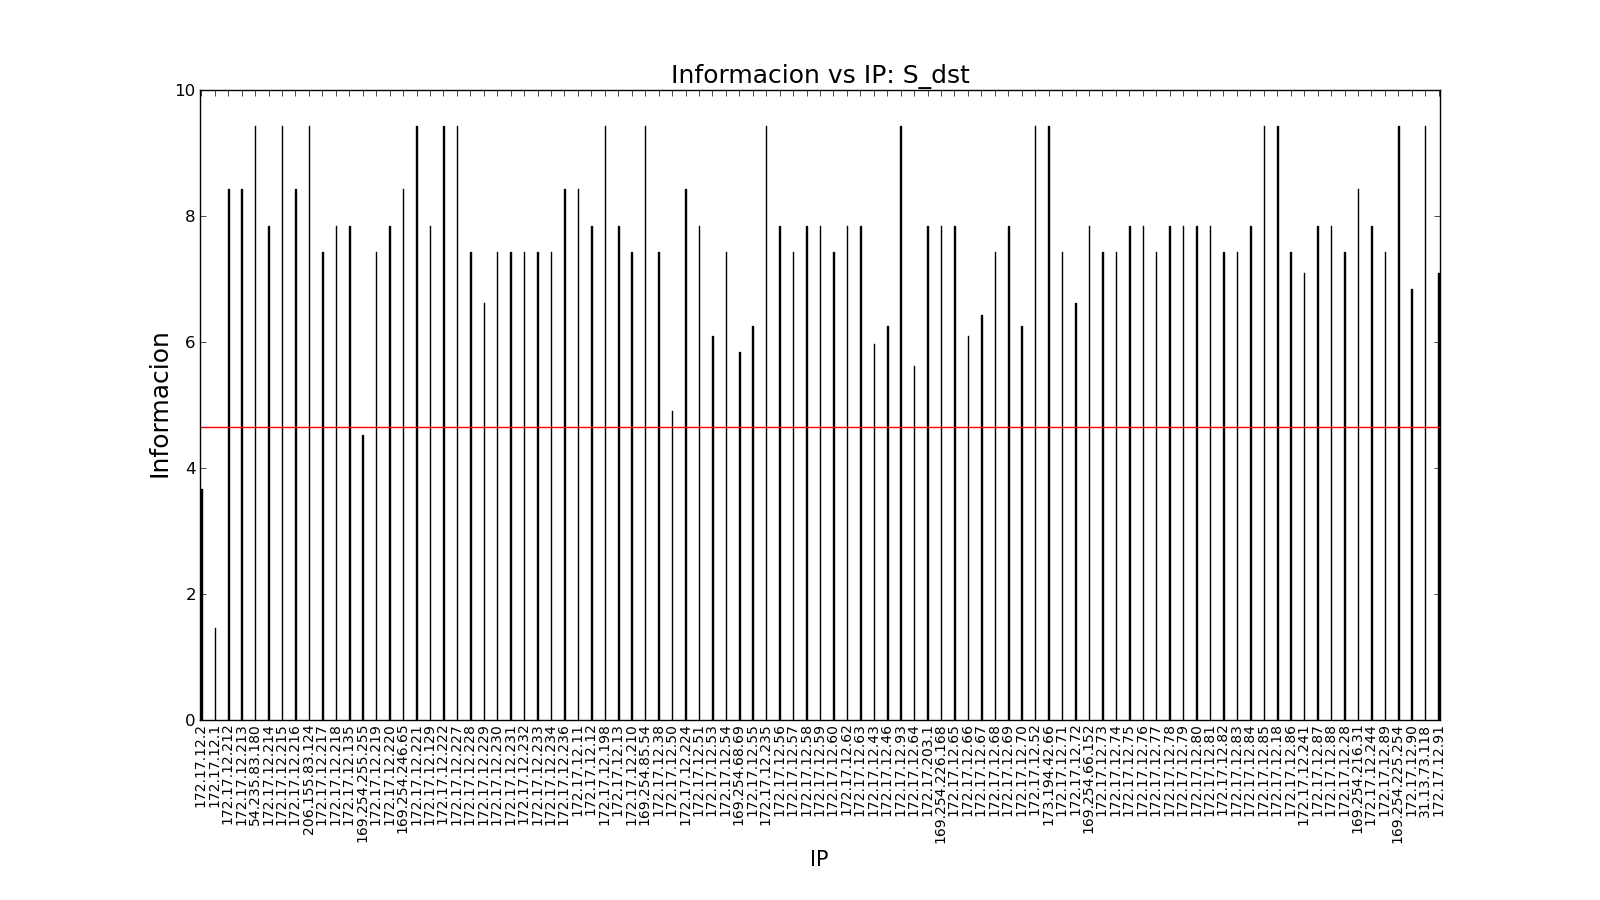
\includegraphics[width=0.8\linewidth]{../imgs/red-alto-palermo_S_dst_info.png}
  \caption{Informacion de $S_{dst}$}\label{fig:Alto-dst-info}
\end{figure}

$\bullet$ Entropía de la fuente: 4.65701881033

Como podemos observar en el primer gráfico, la dirección IP \emph{172.17.12.1} aparece muchas más veces que el resto de las IP. Esto es así porque dicha dirección recibe mensajes de casi todos los demás nodos de la red. Los nodos con direcciónes \emph{172.17.12.2} y \emph{169.254.255.255} también se destacan en el gráfico.

En el segundo gráfico podemos ver que la cantidad de información que aporta la dirección IP \emph{177.17.12.1} es más baja que la entopía de la fuente, al igual que la de las direcciones \emph{172.17.12.2} y \emph{169.254.255.255}.

\subsubsection{Fuente: $S_{src}$}

A contincuación mostramos gráficos similares, pero esta vez para la fuente $S_{src}$:

\begin{figure}[H]\centering
    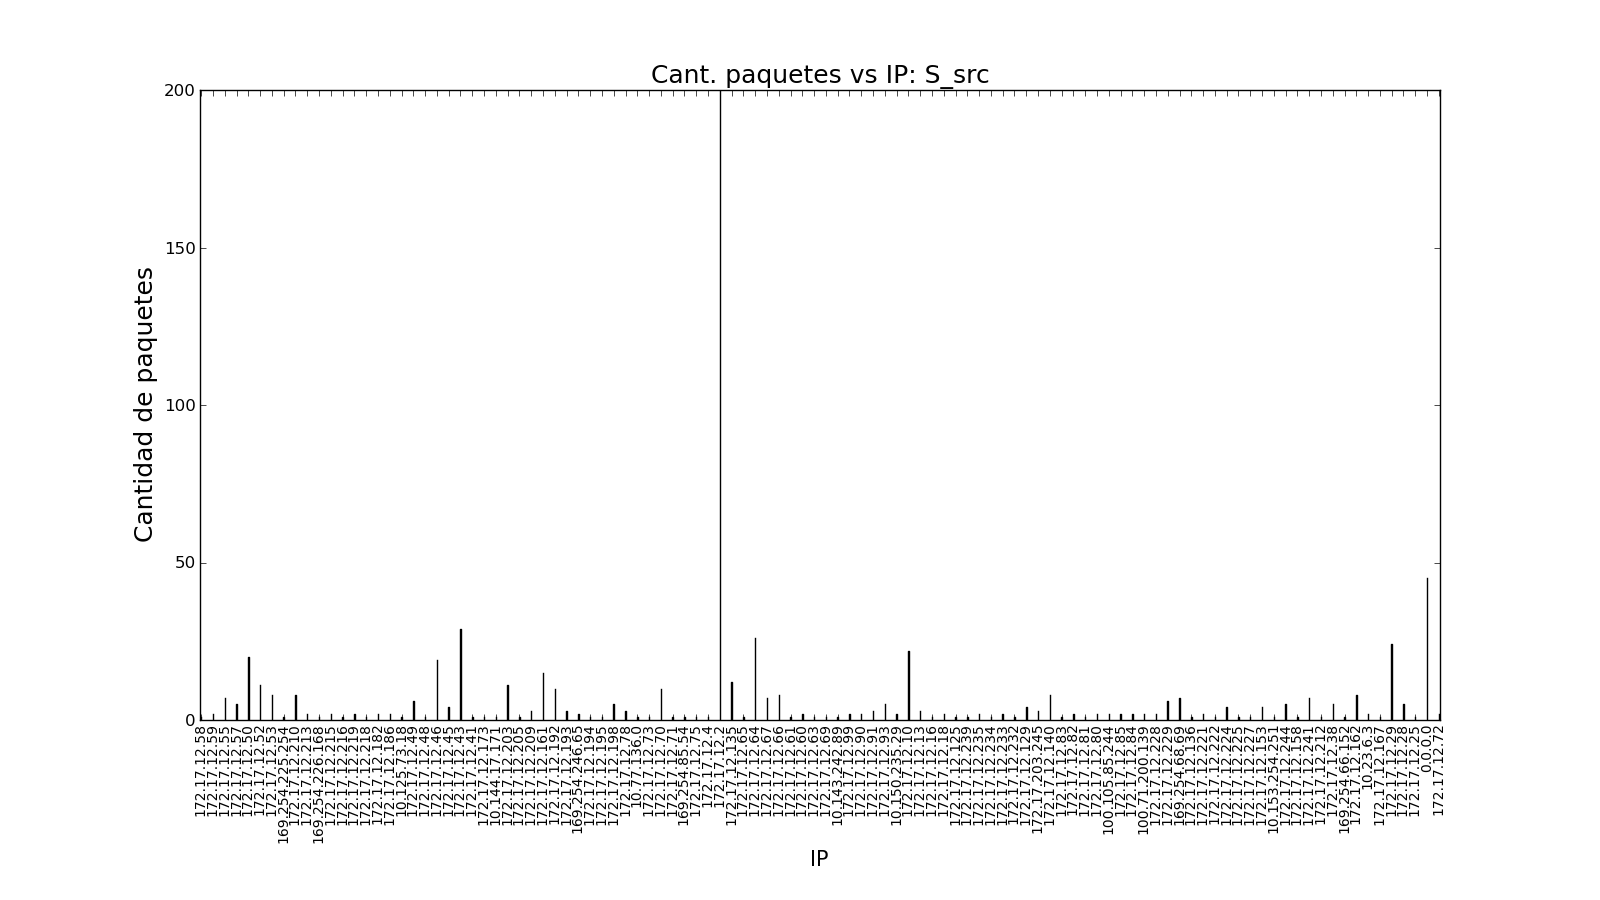
\includegraphics[width=0.8\linewidth]{../imgs/red-alto-palermo_S_src_hist.png}
    \caption{Histograma de $S_{src}$}\label{fig:Alto-src-hist}
\end{figure}

\begin{figure}[H]\centering
    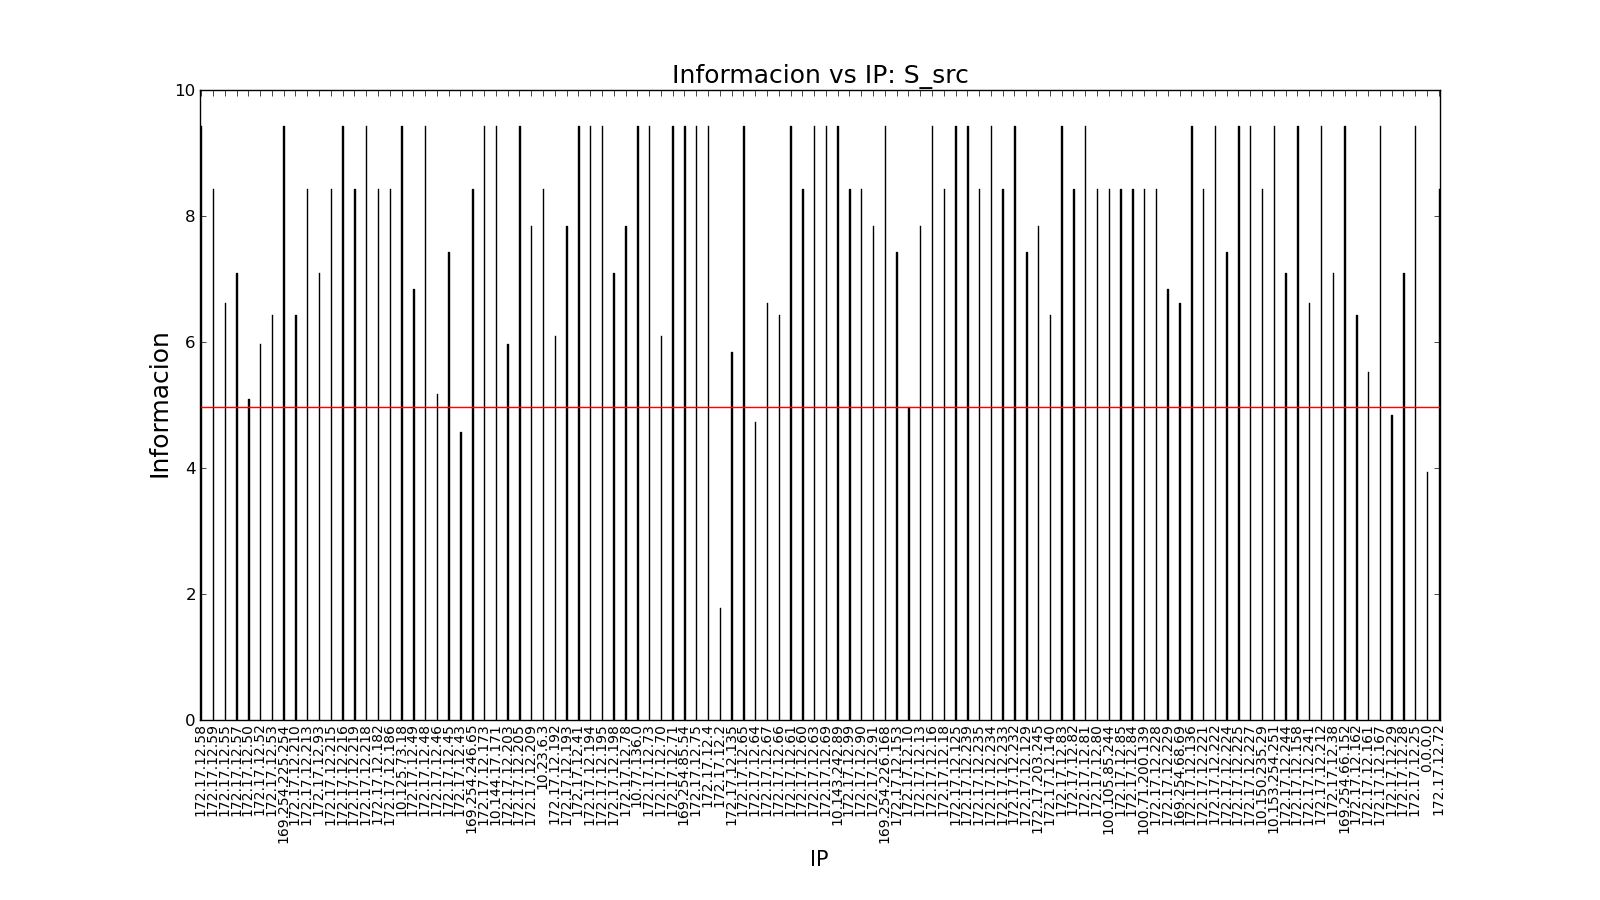
\includegraphics[width=0.8\linewidth]{../imgs/red-alto-palermo_S_src_info.png}
    \caption{Informacion de $S_{src}$}\label{fig:Alto-src-info}
\end{figure}

$\bullet$ Entropía de la fuente: 4.96088403083

En el segundo gráfico podemos observar que hay 5 nodos que aportan menos información que la entropía de la fuente. Estos tienen las direciones \emph{172.17.12.1}, \emph{172.17.12.45}, \emph{172.17.12.64}, \emph{172.17.12.29} y la \emph{0.0.0.0}. 

En el primer gráfico podemos observar que el nodo que tiene la dirección IP \emph{172.17.12.2} envía muchos más paquetes que el resto de los nodos. 

\subsubsection{Discusión}

Suponemos que la dirección \emph{172.17.12.1} es el router de la red ya que es el que aparece como dirección destino en la mayor parte de paquetes \emph{who-has}. Algo que nos llamó la atención es que aparece la dirección \emph{0.0.0.0} como dirección fuente en varios mensajes. Lamentablemente no pudimos saber a que se debe esto.
Además creemos que la dirección \emph{169.254.255.255} es una dirección \emph{broadcast}, ya que su dirección termina con 255.255 y aparece como dirección destino en muchos paquetes (es un nodo distinguido de la fuente $S_{dst}$.
Sin embargo, no pudimos ver qué rol ocupa el nodo con dirección \emph{172.17.12.2}

% %
% Cuando observamos el grafo en la primera parte del análisis de esta red, dijimos que había dos nodos que se destacaban visualmente, los cuales eran los que tenían las direcciones IP \emph{172.17.12.1} y \emph{172.17.12.2}. Al ver el grafo notamos que la mayor parte de los paquetes capturados eran enviados o recibidos por alguno de estos dos nodos. Esto nos hizo suponer que éstos eran dos nodos distinguidos de la red.
% 
% Luego observamos el histograma y el gráfico de barras de la fuente $S_{dst}$. De esta forma vimos que efectivamente el nodo con la IP \emph{172.17.12.1} aparecía como dirección destino en muchos mensajes. Sin embargo el nodo \emph{172.17.12.2} no aparecía tantas veces.
% 
% Al hacer lo mismo con la fuente $S_{src}$ notamos que el nodo que aparecía más veces era el nodo \emph{172.17.12.2}. El nodo \emph{172.17.12.1} no era un símbolo de $S_{src}$ ya que éste no mandó mensajes, por lo tanto no aparece en estos gráficos.
% 
% Concluimos entonces que el nodo de la red que tiene la dirección IP \emph{172.17.12.1} se trata de un nodo distinguido, el cual creemos que es el router de la red. Sin embargo, no pudimos ver qué rol ocupaba el nodo \emph{172.17.12.2} en la misma.